\chapter{Reproducing \tfunet}
\label{ch:tfunet}

\section{Results on Synthetic Data}
We applied the \tfunet{} code of Akeret et al.\footcite{akeret2017}, which is
publicly available on GitHub, to the 276$\times$600 version of our synthetic
data, the image size used by the authors. The network was used unchanged
(3 levels, 32 filters in the first layer, 465{,}986 parameters), together with
the authors' preprocessing: every image is scaled with one fixed intensity
range, and no class weighting is used. Only the batch size and the optimiser
were adapted to our GPU (\cref{sec:tfunet_setup}). On the synthetic test set
\tfunet{} reached a maximum \Fone{} of 0.9317, with a ROC AUC of 0.9908.

\section{Results on LOFAR}
\label{sec:tfunet_lofar}
We then trained \tfunet{} on the real LOFAR data with the same settings: the
unmodified network, fixed-range normalisation and no class weighting. The model was trained on the
6621 clean training images, the threshold was chosen on 150 of the 735
validation images, and the result was measured on the 109 images labelled by the human
expert. Each setting was run with three random seeds.

Despite the extreme imbalance---one RFI pixel for every 129 clean ones---the
network did not collapse into predicting ``no RFI'' everywhere. With the same
training length as on the synthetic data (60 epochs at a learning rate of
$10^{-3}$) it reached a maximum \Fone{} of $0.4901 \pm 0.0495$. Lowering the
learning rate to $10^{-4}$ and training for 150 epochs raised this to
$0.5482 \pm 0.0139$ (\cref{tab:tfunet_lofar}).

\begin{table}[H]
  \centering
  \caption[\tfunet{} results on LOFAR]{\tfunet{} on the 109 human-labelled LOFAR test images. Mean and
    standard deviation over three seeds.}
  \label{tab:tfunet_lofar}
  \begin{tabular}{lccc}
    \toprule
    Training & max \Fone{} & pooled \Fone{} & ROC AUC \\
    \midrule
    lr $10^{-3}$, 60 epochs  & $0.4901 \pm 0.0495$ & $0.4563 \pm 0.0279$ & $0.9389 \pm 0.0045$ \\
    lr $10^{-4}$, 150 epochs & $0.5482 \pm 0.0139$ & $0.5021 \pm 0.0259$ & $0.9470 \pm 0.0074$ \\
    \bottomrule
  \end{tabular}
\end{table}

The lower learning rate also made the result much more consistent between
seeds: the standard deviation of the maximum \Fone{} fell from 0.0495 to
0.0139.

\Cref{fig:tfunet_lofar} places the result among published methods. The values
for Mesarcik et al.'s U-Net and for RFI-Net are as reported in their
paper\footcite{mesarcik2022}. Their results are reported as maximum \Fone{},
which is why that measure is used here. \tfunet{} clearly beats a simple
$\sigma$-clipping threshold (0.4103) but stays below \aoflagger{} (0.5698), and
is 0.039 below the U-Net of Mesarcik et al.\ (0.5876). The two are not the same
network: Mesarcik et al.\ used their own implementation of a U-Net, with batch
normalisation and same padding, trained on 32$\times$32 patches, whereas
\tfunet{} is Akeret et al.'s original code, trained here on full images. The two
results therefore compare two different U-Net implementations, not the same one.

\begin{figure}[H]
  \centering
  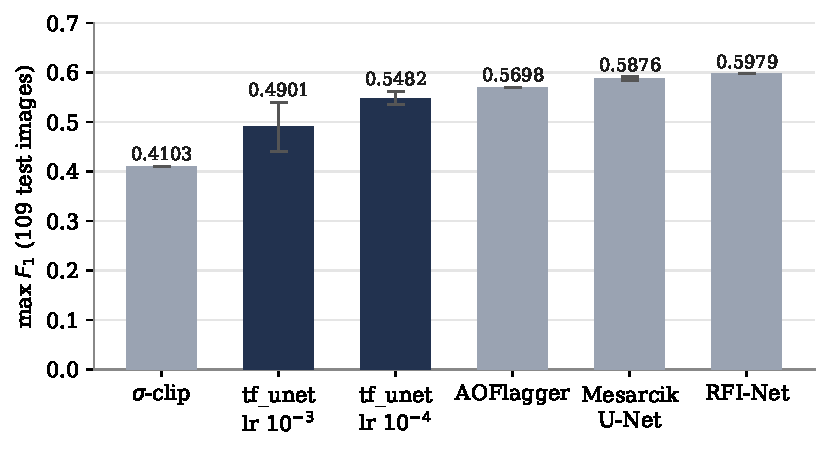
\includegraphics[width=0.8\textwidth]{tfunet_lofar_ladder}
  \caption[\tfunet{} compared with published methods on LOFAR]{Maximum \Fone{} on the 109 LOFAR test images. Dark bars are our
    \tfunet{} runs (error bars: standard deviation over three seeds); grey bars
    are a $\sigma$-clipping threshold, \aoflagger{}, and the values reported by
    Mesarcik et al.}
  \label{fig:tfunet_lofar}
\end{figure}

\subsection{Running Mesarcik et al.'s own code}
\label{sec:mesarcik_rerun}
Mesarcik et al.\ released their code on GitHub\footnote{\url{https://github.com/mesarcik/RFI-NLN}}.
To check their U-Net result, we ran their released code with exactly their
settings: their U-Net, all 7500 training images cut into 32$\times$32 patches,
a batch of 1024 patches, the Adam optimiser with its default settings, 100
epochs, their preprocessing, the model after the last epoch, and the maximum
\Fone{} over all thresholds. This gave a maximum \Fone{} of 0.6207 (one run),
0.033 \emph{above} their published 0.5876. Their code trains on all 7500
images, which include the 109 test images (\cref{sec:lofar_audit}); with these
removed, and the preprocessing computed without the test labels, the result was
0.6166.

We could not find the reason for this difference. The following were checked
and ruled out:
\begin{itemize}
  \item \textbf{Data and score.} Our \aoflagger{} score matches theirs to four
    decimal places, so the test images, labels and \Fone{} calculation are the
    same.
  \item \textbf{Code version.} Their code was changed shortly after the paper
    appeared. The earlier version, which matches the paper's text, gave 0.6258;
    the network itself is identical in both versions.
  \item \textbf{Training details.} Copying their exact way of shuffling the
    training patches and their number precision gave 0.6220.
  \item \textbf{Stopping point.} The score was between 0.62 and 0.63 at every
    5-epoch check from epoch 5 to 100, so stopping earlier or later would not
    have given 0.5876 either.
  \item \textbf{Software version.} They used an older version of TensorFlow
    and Keras. Repeating the run with Keras 2, as they used, instead of Keras 3
    changed the score by less than 0.003.
\end{itemize}
The remaining possible reasons could not be tested: their published runs may
have used a version of the code or data that is not in their public repository,
or differences in their older software and hardware may matter. It is also
possible that their table contains a typing error, since the \Fone{} entry for
the U-Net is printed without the $\pm$ sign and with the same spread (0.0031) as
the AUPRC entry in the same row. All our runs of their code lie between 0.617
and 0.626.


\section{From synthetic to real data}
\label{sec:gap}
The same network, trained with the same settings and the same number of
gradient steps (10{,}500), scores 0.9317 on the synthetic data and 0.4901 on
LOFAR: a drop of 0.44 in \Fone{}. Even the best LOFAR result, after tuning the
learning rate, is 0.38 below the synthetic score. The reasons were set out in
\cref{sec:lofar_harder}: real RFI is far rarer, much of it is fainter than the
noise, and the training labels themselves are often wrong. A method that
performs well on a synthetic benchmark can therefore perform much worse on
real observations, and synthetic results alone should be read with care.
